\documentclass[paper=letter, fontsize=11pt]{scrartcl}

\usepackage{geometry}
\usepackage[T1]{fontenc}
\usepackage{graphicx}
\usepackage[utf8]{inputenc}
\usepackage[spanish, english]{babel}
\usepackage{hyperref}
\usepackage[backend=bibtex, style=trad-abbrv]{biblatex}
\usepackage{sectsty}

\addbibresource{bibliography.bib}

\geometry{
  top=1in,
  right=1in,
  left=1in,
  bottom=1in
}

\allsectionsfont{\raggedright\large \textit\normalfont\scshape\emph}

\title{
  \normalsize
  Challenges in Automatic Meme Generation Using Deep Neural Networks
}

\begin{document}

\maketitle

\section*{Introduction}

\noindent
Today's Internet is full of \textbf{memes}: small chunks of data which represent a large proportion\
of a social network's communication ``protocol''. As coined by Dawkins in his 1976 book\
\emph{``The Selfish Gene''} \cite{dawkins2006}, the meme is the fundamental building-block of information whose behavior seems very likely to that of a gene (\emph{better} memes tend to prevail longer in the Internet).\
Also, there is an evolution mechanism that allows older memes to adapt to current trends.\par
In this project, the problem of learning representations from a meme dataset and immediately generating new\
data is studied, as a basis to motivate the further study of memes using \emph{state-of-the-art} machine\
learning methods. In particular, we develop a deep neural architecture which attempts to learn a language\
model out of a dataset of plain meme images along with several associated captions.\par
Much of deep learning's success is justified by the outstanding performance of Vinyals', \textit{et al},\
\textbf{Show-and-Tell model} \cite{DBLP:journals/corr/VinyalsTBE14}. We report experiments directly\
using such model, in comparison with a proposed model that uses a \emph{more shallow} convolutional network.

\begin{figure}[h]
    \centering
    \begin{minipage}[l]{0.2\linewidth}
    
\includegraphics[width=\linewidth]{img/meme2.jpg}
    \end{minipage}\hfill
    \begin{minipage}[r]{0.2\linewidth}
    
\includegraphics[width=\linewidth]{img/meme3.jpg}
    \end{minipage}\hfill
    \begin{minipage}[r]{0.2\linewidth}
    
\includegraphics[width=\linewidth]{img/meme4.jpg}
    \end{minipage}\hfill
    \begin{minipage}[r]{0.2\linewidth}
    
\includegraphics[width=\linewidth]{img/meme6.jpg}
    \end{minipage}
	\caption{
        Meme examples. Most of them were 
        popular between 2009 and 2013, yet some of them have evolved!
        (Image taken from \url{https://memegenerator.net}.)
    }
    \label{fig1}
\end{figure}
As pointed out by Figure \ref{fig1}, we choose to start with memes that mainly consist on an\
image centered on a main character and a caption. We, finally, report some evaluation measurements\
to analyze our architecture's performance.\par
This project was mainly presented as an undergraduate thesis \cite{tes.TES0100077017320180101}, under the supervision of\
\href{http://turing.iimas.unam.mx/~ivanvladimir/}{Dr Ivan Vladimir Meza Ruiz}. A similar work was described later in \cite{2018arXiv180604510P}.\par
Formally, we trained our architecture with data samples consisting of $(I, S)$ tuples,\
where $I$ is an image and $S$ is the set of its associated captions.\
We used $70\%$ of our dataset for training and the remaining for testing. We use the\
original \emph{Show-and-Tell} model, at first, to see how it would perform with a much smaller dataset\
than \emph{ImageNet}. Then we, conjectured that a shallow convolutional network could do better; thus,\
we trained the model shown in Figure \ref{fig3}.  
The CNN extracted output was inserted as \emph{initial state} to a LSTM\
recurrent network, whose training resembled what is defined on \cite{DBLP:journals/corr/VinyalsTBE14}.

\section*{Lessons}

\noindent
The proposed neural architecture provides a baseline to work with many tasks related with learning representations from raw Internet memes. We achieved, at a high level, a significant performance when evaluating the generated captions using a perplexity measurement against a testing meme dataset%
\footnote{
    Such testing dataset was built upon cross validation splitting the crawled data, and only considering captions but not images.
}. Furthermore, it is expected that this step, with some refinements, may be useful to train language-specific datasets.\par
In terms of image classification, our good results in pre-training imply the possibility of adding broader convolutional networks to the proposed pipeline. Thus, one can think of refining our classification (i.e., getting better feature vectors), prior getting into the recurrent network.

\section*{Challenges}

\begin{itemize}
    \item Any pipeline must get used to new formats, whose origin doesn't necessarily come from websites dedicated to construct a meme, but from any social network. 
    \item Bring together a more thorough and diverse dataset that includes novel meme designs. This is especially useful (and necessary) to what was specified on the previous section. A hierarchical classification of memes, such as what ImageNet does, might be extremely useful, as well.
    \item Accurate evaluation metrics are still missing, for our current methods only consider language model-based similarities, through the use of perplexities. In this case, a thorough methodology must be built, including scoring by humans, considering that humour is a very ambiguous concept.
    \item It would rather be interesting to experiment with formats that include comic-like structures or a certain sequence. In such cases, a recurrent architecture might be helpful, to be combined with CNN's.
    \item Humour varies, roughly, between countries. For instance, in Mexico, the reasons a meme reaches a level of popularity depends of very different social media actors than those who influence the American "meme market". Thus, it is critical to include an attention mechanism and link it with a context representation out of actual social media trends.
\end{itemize}

%% \nocite{*}
\printbibliography[title={Bibliography}]

\appendix{Appendix A: Neural Architecture}

  \begin{figure}[h]
    \centering
    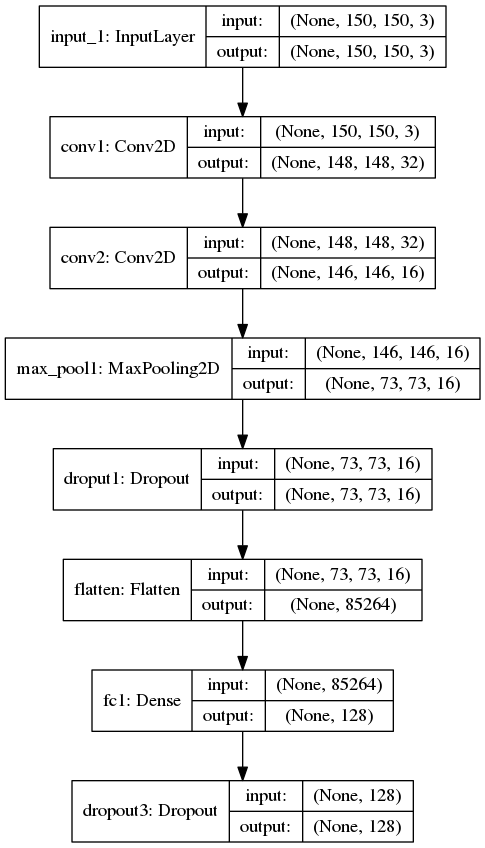
\includegraphics[width=0.45\linewidth]{img/model.png}
    \caption{
        A shallow architecture used to extract convolutional feature maps from a crawled dataset.
    }
    \label{fig3}
\end{figure}

\end{document}
